\documentclass[../Cours.tex]{subfiles}

\begin{document}
\chapitre{Périmètres}

\partie{Cas général}

\definition{Le périmètre d'une figure est la longueur de son contour.}

\exemple{
    \begin{center}
    \begin{tikzpicture}[scale=0.6]
        \draw[noir,gray!80!white] (0,0) grid (6,5);
        \draw[rouge, line width={0.5mm}] (1,1) -- (1,4) -- (3,4) -- (3,2) -- (4,2) -- (4,3) -- (5,3) -- (5,1) -- cycle;
        \draw[rouge, line width={0.2mm},latex-latex] (5.3,2) -- (5.3,1);
        \node[rouge, anchor=west] at (5.3,1.5) {\scriptsize{unité de longueur}};
        \node at (3,-1) {Le périmètre de cette figure est de 16 unités de longueur.};
    \end{tikzpicture}
    \end{center}
}

\propriete{Le périmètre d'un polygone est égal à la somme des longueurs de ses côtés.}

\remarque{Bien vérifier que toutes les longueurs soient exprimées dans la même unité.}

\exemple{
    \begin{center}
    \begin{tikzpicture}
        \coordinate (A) at (0,0);
        \coordinate (B) at (4,-0.8);
        \coordinate (C) at (3,2);
        \coordinate (D) at (0.5,2.5);
        \draw (0,0) node[left]{$A$} -- (4,-0.8) node[right]{$B$} -- (3,2) node[right]{$C$} -- (0.5,2.5) node[left]{$D$} -- cycle;
        \node[anchor=west] at (-5,-2) {$\curs{P}_{ABCD} = AB+BC+CD+DA=\qty{3}{\centi\metre}+\qty{2}{\centi\metre}+\qty{2.4}{\centi\metre}+\qty{1.6}{\centi\metre}$};
        \node[anchor=west] at (-5,-3) {$\curs{P}_{ABCD} = AB+BC+CD+DA=\qty{9}{\centi\metre}$};
        \node[below] at ($(A)!0.5!(B)$) {\qty{3}{\centi\metre}};
        \node[right] at ($(B)!0.5!(C)$) {\qty{2}{\centi\metre}};
        \node[above] at ($(C)!0.5!(D)$) {\qty{2.4}{\centi\metre}};
        \node[left] at ($(D)!0.5!(A)$) {\qty{1.6}{\centi\metre}};
    \end{tikzpicture}
    \end{center}
}

\partie{Formules}
\souspartie{Polygones}

\begin{center}
    \begin{tabularx}{0.9\linewidth}{|l|C|C|C|}\hline
         & Rectangle & Losange & Carré \\\hline
        Figure & \makecell{
        \begin{tikzpicture}[scale=1.2]
            \draw (0,0) rectangle (2,1);
            \node at (1,0) {||};
            \node at (1,1) {||};
            \node at (0,0.5) {*};
            \node at (2,0.5) {*};
            \draw[latex-latex] (2.3,0) -- (2.3,1) node[midway,right]{$\ell$};
            \draw[latex-latex] (0,-0.4) -- (2,-0.4) node[midway,below]{$L$};
        \end{tikzpicture}
        } & \makecell{
        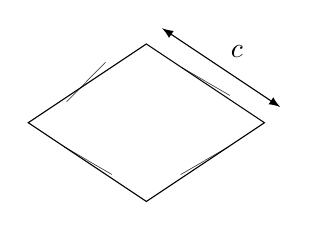
\begin{tikzpicture}
            \draw (0,0) -- (1.5,1) node[midway,rotate=45]{||} -- (3,0) node[midway,rotate=-30]{||} -- (1.5,-1) node[midway,rotate=30]{||} -- cycle node[midway,rotate=-30]{||};
            \draw[latex-latex] (1.7,1.2) -- (3.2,0.2) node[midway,above right]{$c$};
        \end{tikzpicture}
        } & \makecell{
        \begin{tikzpicture}
            \draw (-0.75,-0.75) rectangle (0.75,0.75);
            \node at (0,-0.75) {+};
            \node at (0,0.75) {+};
            \node at (-0.75,0) {+};
            \node at (0.75,0) {+};
            \draw[latex-latex] (1,-0.75) -- (1,0.75) node[midway,right]{$c$};
        \end{tikzpicture}
        } \\\hline
        Formule & $2 \times L + 2 \times \ell$ & $4 \times c$ & $4 \times c$ \\\hline
    \end{tabularx}
\end{center}

\souspartie{Cercle}

\propriete{Le périmètre d'un cercle de rayon $r$ se calcule grâce à la formule : $2 \times \pi \times r$.}

\exemple{Calculer le périmètre d'un cercle de rayon \qty{5}{\centi\metre}.
$$ \curs{P}_{\mbox{cercle}} = 2 \times \pi \times \qty{5}{\centi\metre} \approx \qty{31.4}{\centi\metre}$$
Calculer le périmètre d'un quart de cercle de rayon \qty{3}{\centi\metre}.
$$ \curs{P}_{\mbox{quart de cercle}} = \dfrac{1}{4} \times \curs{P}_{\mbox{quart de cercle}} = \dfrac{1}{4} \times 2 \times \pi \times \qty{3}{\centi\metre} \approx \qty{4.71}{\centi\metre} $$
}



\end{document}